We deployed rsMPI on a cluster of 30 nodes (600 cores) for testing and benchmarking. Each node consists of a 2-way SMPs with Intel Haswell E5-2660 v3 processors of 10 cores per socket (20 cores per node), and is configured with 128 GB RAM. Nodes are connected via 56 GB/s FDR InfiniBand. %To maximize the compute capacity, we used up to 20 cores per node.

Benchmarks from the Sandia National Lab Mantevo Project and NAS Parallel Benchmarks (NPB) are used. %, and evaluated rsMPI with various problem sizes and number of processes. 
CoMD is a proxy for molecular dynamics application. MiniAero is an explicit unstructured finite volume code that solves the Navier-Stokes equations. Both MiniFE and HPCCG are unstructured implicit finite element codes, but HPCCG uses MPI\_ANY\_SOURCE receive operations and can demonstrate rsMPI's capability of handling non-deterministic events. IS, EP, and CG from NPB represent integer sort, embarrassingly parallel, and conjugate gradient applications, respectively. These applications cover key simulation workloads and represent both different communication patterns and computation-to-communication ratios.

We also implemented in-memory checkpointing~\cite{zheng2004ftc} to compare with rsMPI in the presence of failures. 
%To be optimistic, we chose double in-memory checkpointing that is much more scalable than disk-based checkpointing~\cite{zheng2004ftc}. 
Same as leaping in rsMPI, our application-level checkpointing provides an API for process state registration. This API requires the same parameters, but internally, it allocates extra memory in order to store the state of a ``buddy" process. Another provided API is checkpoint(), which inserts a checkpoint in the application code. For fairness, MPI messages are used to transfer state between buddies.  
For both rsMPI and checkpointing/restart, we assume a 60 seconds rebooting time after a failure. All figures in this section show the  average of 5 runs with the standard deviation.

\subsection{Measurement of runtime overhead}
\label{sec:runtime_overhead}
While the hardware overhead for rsMPI is straightforward, 
%(e.g., collocation ratio of 4 results in the need for 25\% more hardware cost), 
the runtime overhead of the enforced consistency protocol depend on applications. To measure this overhead we ran each benchmark application linked to rsMPI and compared the execution time with the baseline, where each application runs with unmodified OpenMPI.

Figure~\ref{fig:runtime_overhead} shows the comparison of the execution time for the 7 applications in the absence of faults. All the experiments are conducted with 256 application-visible processes. That is, the baseline uses 256 MPI ranks, while rsMPI uses 256 mains together with 256 shadows. %Each result shows the average execution time of 5 runs, the standard deviation, and rsMPI's runtime overhead. %The baseline execution time varies from seconds to half an hour, so we plotted the time in log-scale. 
From the figure we can see that rsMPI has comparable execution time to the baseline for all applications except IS. The reason for the exception is that IS uses all-to-all communication and is heavily communication-intensive. %This is verified by adding fake computation to the application and we can see an immediate drop of the overhead to negligible level. 
We argue that communication-intensive applications like IS are not scalable, and as a result, they are not suitable for large-scale HPC. 
For all other applications, the overhead varies from 0.64\% (EP) to 2.47\% (CoMD). %Even for HPCCG, which uses MPI\_ANY\_SOURCE and adds extra work to our consistency protocol, the overhead is only 1.95\%, thanks to the asynchronous semantics of MPI\_Send. 
Therefore, we conclude that rsMPI's runtime overheads are modest for applications that exhibit a fair communication-to-computation ratio.

\begin{figure}[!t]
  \begin{center}
      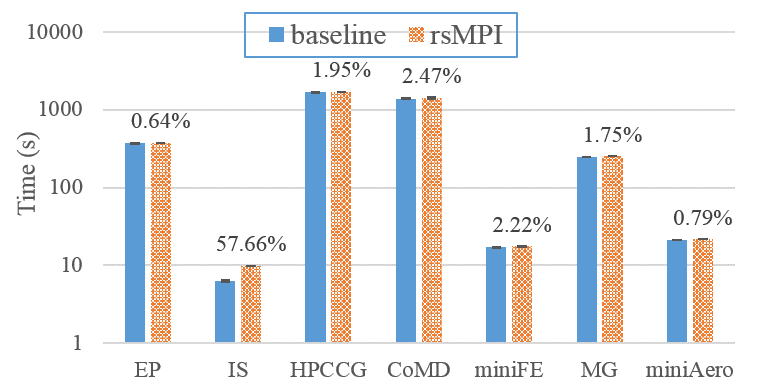
\includegraphics[width=0.9\columnwidth]{Figures/runtime_overhead_hpcc}
  \end{center}
  \vskip -0.1in
  \caption{Comparison of execution time between baseline and rsMPI using 256 application-visible processes and collocation ratio of 2 for rsMPI.}
  \label{fig:runtime_overhead}
  %\vspace{-0.05in}
\end{figure}

\subsection{Scalability}
%In addition to measuring the runtime overhead at fixed application-visible process count, we also assessed both strong and weak scalability by varying the number of processes for the applications. Strong scaling is defined as how the execution time varies with the number of processes for a fixed total problem size. In contrast, weak scaling is defined as how the execution time varies with the number of processes for a fixed problem size per process.

%In addition to measuring the runtime overhead at fixed process count, 
We also assessed the applications' weak scalability, which measures how the execution time varies with the number of processes for a fixed problem size per process.
Among the seven applications, HPCCG, CoMD, and miniAero allow us to configure the input for weak scaling test. The results for miniAero are similar to those of CoMD, so we only show the results for HPCCG and CoMD in Figure~\ref{fig:scalability}. %Figure~\ref{fig:scalability} reveals that both HPCCG and CoMD have good strong scalability. By increasing the number of processes, we can always reduce the execution time for a fixed problem size. At the same time, rsMPI's runtime overhead increases with the number of processes during the strong scalability test. At 256 processes, the overhead reaches 13.2\% for CoMD, and 29.1\% for HPCCG. This may seem to contradict with the results in Section~\ref{sec:runtime_overhead}. It is expected, however, since increasing the number of processes while keeping a constant problem size increases the communication-to-computation ratio of the application. Hence, to keep rsMPI overheads reasonable, it is important to choose input sizes such that the ratio of communication-to-computation is balanced. 


\begin{figure}[!t]
	\begin{center}
		\subfigure[HPCCG weak scalability]
		{
			\label{fig:hpccg_weak}
			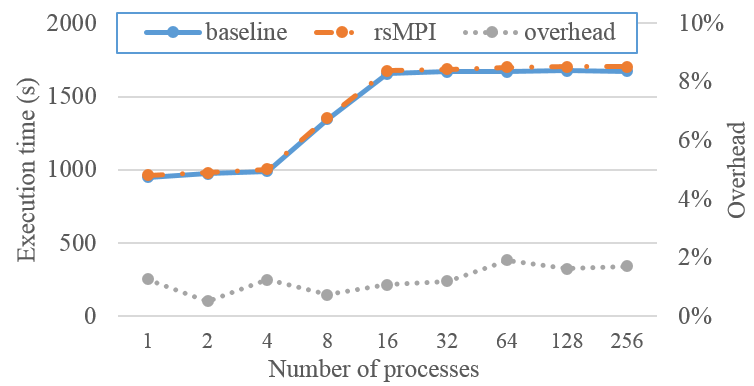
\includegraphics[width=0.9\columnwidth]{Figures/hpccg_weak_hpcc}
		}
		\subfigure[CoMD weak scalability]
		{
			\label{fig:comd_weak}
			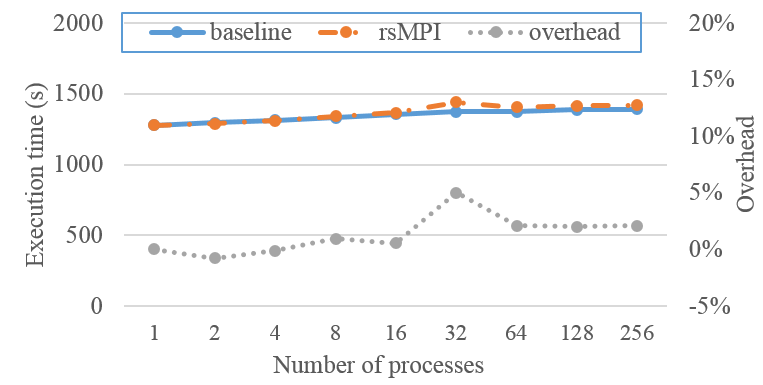
\includegraphics[width=0.9\columnwidth]{Figures/comd_weak_hpcc}
		}
	\end{center}
	\vskip -0.2in
	\caption{Scalability test for number of processes from 1 to 256. Collocation ratio is 2 for rsMPI.}
	\label{fig:scalability}
    \vspace{-0.2in}
\end{figure}

Comparing between Figure~\ref{fig:hpccg_weak} and Figure~\ref{fig:comd_weak}, it is obvious that HPCCG and CoMD have different weak scaling characteristics. While the execution time for CoMD increases by 8.9\% from 1 process to 256 processes, the execution time is almost doubled for HPCCG. However, further analysis shows that from 16 to 256 processes, the execution time increases by only 2.5\% for CoMD, and 1.0\% for HPCCG. We suspect that the results are not only affected by the scalability of the application, but also impacted by other factors, such as cache and memory contention on the same node, and network interference from other jobs running on the cluster. %Note that each node in the cluster has 20 cores and we always use all the cores of a node before adding another node. Therefore, it is very likely that the node level contention leads to the substantial increase in execution time for HPCCG. The results from 16 to 256 processes show that both HPCCG and CoMD are weak scaling applications. 
To predict the overhead at exascale, we applied curve fitting to derive the correlation between runtime overhead and the number of processes. At $2^{20}$ processes, it is projected that the overhead is 3.1\% for CoMD and 7.6\% for HPCCG. 

%Similar to the results of the previous section, the runtime overhead for rsMPI is modest. The maximum overhead observed is 5.0\% when running CoMD with 32 processes. Excluding this case, the overhead is always below 2.1\%. To predict the overhead at exascale, we applied curve fitting to derive the correlation between runtime overhead and the number of processes. At $2^{20}$ processes, it is projected that the overhead is 3.1\% for CoMD and 7.6\% for HPCCG. 

%Different from strong scalability test, there is no correlation between rsMPI's runtime overhead and the number of processes during the weak scalability test. The overhead is always below 2.1\%, except for the case of 32 processes for CoMD where the overhead is 5.0\%. %The reason for this exception is still under investigation.

\subsection{Performance under failures}
%The last set of experiments test rsMPI's capability of tolerating failures and evaluate its performance under various failures by comparing with checkpointing/restart. 

As one main goal of this work is to achieve fault tolerance, an integrated fault injector is required. % to evaluate the effectiveness and efficiency of rsMPI to tolerate failures during execution. 
To produce failures in a manner similar to naturally occurring process failures, the failure injector is designed to be distributed and co-exist with all rsMPI processes. Failure is injected by sending a specific signal to a randomly picked target process.

We assume that the underlying hardware platform has a Reliability, Availability and Serviceability (RAS) system that provides failure detection. In our test system, we emulate the RAS functionality by associating a signal handler with every process. The signal handler catches failure signals sent from the failure injector, and uses a rsMPI defined failure message via a dedicated communicator to notify all other processes.% of the failure. 
%To detect failure, rsMPI receiving operation checks for failure messages before performing the actual receiving. 
%Similar to ULFM, a process in rsMPI can only detect failure when it posts an MPI receive operation. %In a rsMPI receive, 
%a process checks for failure messages before it performs the actual receive operation.

The first step was to test the effectiveness of leaping. %For each application, we identified the process state and register them with rsMPI. 
Figure~\ref{fig:single_failure} shows the execution time of HPCCG with a single failure injected at a specific time, measured as a proportion of the total execution of the application. %, at an increment of 10\%.
The execution time is normalized to that of the failure-free baseline.   
%with a single failure injected at various locations. 
The blue solid line and red dashed line represent rsMPI with collocation ratio of 2 and 4, respectively. For simplicity, they are referred to as rsMPI\_2 and rsMPI\_4 in the following text.  
%Corresponding to the x-axis, a single failure is injected at various execution time in terms of iterations. For example, 10\% means that the completion of 500 iterations for an application with 5000 iterations in total.
%The blue solid line represents rsMPI without any forced leaping, and the red dash line represents rsMPI with periodic forced leaping. Note that the execution time is reduced compared to previous results because we reduced the number of iterations for the application main loop from 5000 to 150, so that there is no need for any forced leaping by buffer overflow. 
%Every time we set our failure injector to randomly pick a process to inject a failure, and the failure is scheduled to occur at certain point during the execution. Corresponding to the x-axis, the scheduled failure time varies from 10\% to 90\% of the application's execution. For example, 10\% means the application completes 15 iterations for a total of 150 iterations. 

\begin{figure}[!t]
  \begin{center}
      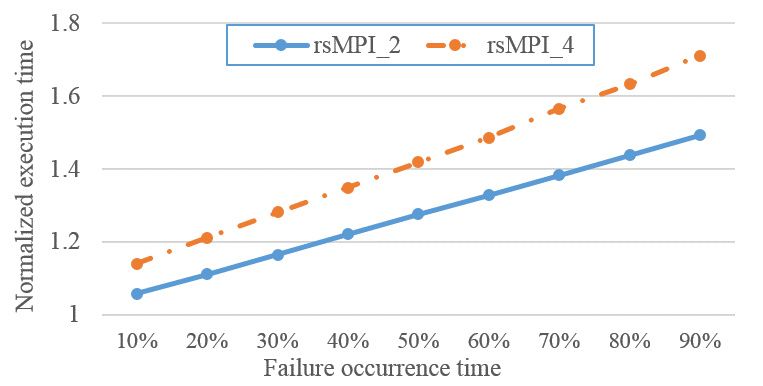
\includegraphics[width=0.9\columnwidth]{Figures/single_failure_hpcc}
  \end{center}
  \vskip -0.2in
  \caption{Execution time of HPCCG with a single failure injected at various time, normalized to that of the failure-free baseline.}
  %\vspace{-10pt}
  \label{fig:single_failure}
\vspace{-0.25in}
\end{figure}

As shown in Figure~\ref{fig:single_failure}, rsMPI's execution time increases with the failure occurrence time, regardless of the collocation ratio. The reason is that recovery time in rsMPI is proportional to the amount of divergence between mains and shadows, which grows with the execution. 
Another factor that determines the divergence is the shadow's execution rate. The slower the shadows execute, the faster the divergence grows. As a result, rsMPI\_2 can recover faster than rsMPI\_4, and therefore achieves better execution time.

%As expected, without forced leaping the execution time increases with the failure occurrence time, as reflected by the blue line in Figure~\ref{fig:single_failure}. The reason is that failure recovery time for rsMPI is proportional to the amount of divergence between mains and shadows, and the divergence grows as the execution proceeds. On the other hand, forced leaping can effectively reduce the divergence by leaping the shadow forward to the state of its associated main, similar to the idea that checkpointing can reduce the amount of wasted work due to a failure by saving the execution state. To prove the effectiveness of leaping, we insert 4 forced leaping at 20\%, 40\%, 60\% and 80\% of the execution. The red line in Figure~\ref{fig:single_failure} clears show that the divergence effect is bounded due to periodic leaping, regardless of the failure occurrence time.

The results in Figure~\ref{fig:single_failure} suggests that rsMPI is better suited to environments where failures are frequent. 
This stems from the fact that, due to leaping, the divergence between mains and shadows is eliminated after every failure recovery. %As the number of failure increases, the interval between failures decreases, thereby reducing the recovery time per failure.
To demonstrate the above analysis, we compare rsMPI with checkpointing under various failure rates. 
To run the same number of application-visible processes, rsMPI needs more nodes than checkpointing to host the shadow processes. 
For fairness, we take into account the extra hardware cost for rsMPI by defining the following metric:
$$\text{Weighted execution time} = T_e \times S_p,$$ where $T_e$ is the wall-clock execution time and $S_p$ is the projected speedup. For example, we measured that the speedup of HPCCG from 128 processes to 256 processes is 1.88, and rsMPI\_2 needs 1.5 times more nodes than checkpointing, so the projected speedup is $1.5\times\frac{1.88}{2}=1.41$. %Similarly, we calculate the projected speedup for rsMPI\_4 as $1.25\times\frac{1.88}{2}=1.17$.
%$$\text{Efficiency} = \frac{T_f \times N}{T_e \times M}$$
%, where $T_f$ and $N$ are the execution time and number of nodes without failures, and $T_e$ and $M$ are the actual execution time and required number of nodes for a specific fault tolerance mechanism. Intuitively, $T_f \times N$ represents the total amount of workload required by the application, and $T_e \times M$ is the actual amount of work carried out. The efficiency will be in the range 0 to 1, inclusive, and the higher is the better.

%The forced leaping interval for an application is selected such that no buffer overflow at the shadows would take place. Therefore, the interval should vary from system to system and also depends on the application patterns. We assume checkpointing/restart has the same buffer pressure as it needs to perform message logging, so its checkpointing interval is selected based on the same metric as rsMPI. We evaluated rsMPI with 2 different collocation ratios, i.e., 2 and 4. When collocation ratio is 2, rsMPI uses 50\% more nodes than checkpointing, and the execution rate of each shadow is roughly 50\% of the processor rate. Therefore, we set the checkpointing interval to be the same as the forced leaping interval for rsMPI. When collocation ratio is 4, rsMPI needs 25\% more nodes, and each shadow's rate is roughly 25\% of the processor rate. As a result, we loose the checkpointing interval to be twice of the forced leaping interval. 

%With the checkpointing and forced leaping inserted to the application code, we randomly injected up to 10 failures into the execution. Figure~\ref{fig:multiple_failure} shows the comparison between checkpointing and rsMPI (collocation ratio of 4) for both execution time and efficiency defined above. Although the failure-free execution time of rsMPI is slightly larger than that of checkpointing, which results from rsMPI's consistency protocol, the failure recovery time of checkpointing immediately overwhelms that of rsMPI as failures occur. With 10 failures, the execution time of checkpointing is 42.8\% more than that of rsMPI. Considering hardware overhead, the efficiency of checkpointing is also worse than that of rsMPI when the number of failures reaches 6.

In this analysis, we set the checkpointing interval to $0.1T$, where $T$ is the total execution time. To emulate failures, for both checkpointing and rsMPI, we randomly inject over $T$ a number of faults, $K$, ranging from 5 to 30. This fault rate corresponds to a processor's MTBF of $NT/K$, where $N$ is the number of processors. %That is, the processor's MTBF is proportional to the total execution time and the number of processors. For example, %when using $256$ processors and executing for $1700$ seconds, injecting $10$ faults corresponds to a processor's MTBF of $12$ hours. However, 
When using a system of $64,000$ processors and executing over $4$ hours, injecting $10$ faults corresponds to a processor's MTBF of $3$ years.

Figure~\ref{fig:multiple_failure} compares checkpointing and rsMPI, based on both wall-clock and weighted execution time. Ignoring the hardware overhead, Figure~\ref{fig:failures_time} shows that, when the number of failures is small (e.g., 5 failures), checkpointing slightly outperforms rsMPI. As the number of failures increases, however, rsMPI achieves significantly higher performance than checkpointing. For example, when the number of failures is 20, rsMPI\_2 saves 28.7\% in time compared to checkpointing. The saving rises up to 39.3\%, when the number of failures is increased to $30$. Compared to checkpointing, rsMPI\_4 reduces the execution time by 19.7\% and 34.8\%, when the number of failures are 20 and 30, respectively. 

\begin{figure}[!t]
  \begin{center}
      \subfigure[Wall-clock execution time]
		{
			\label{fig:failures_time}
			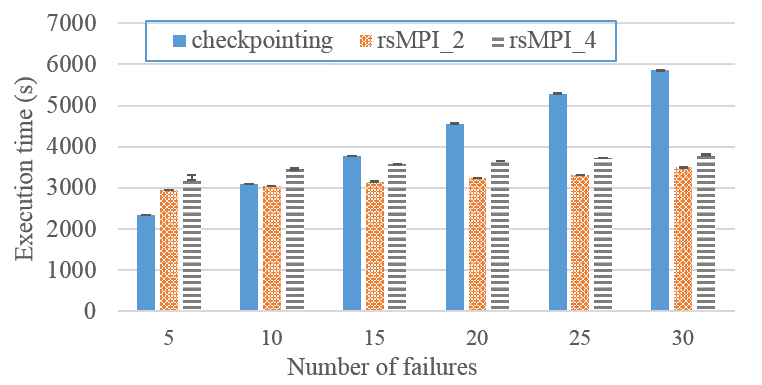
\includegraphics[width=0.9\columnwidth]{Figures/failures_time_hpcc}
		}
		\subfigure[Weighted execution time]
		{
			\label{fig:failures_ntime}
			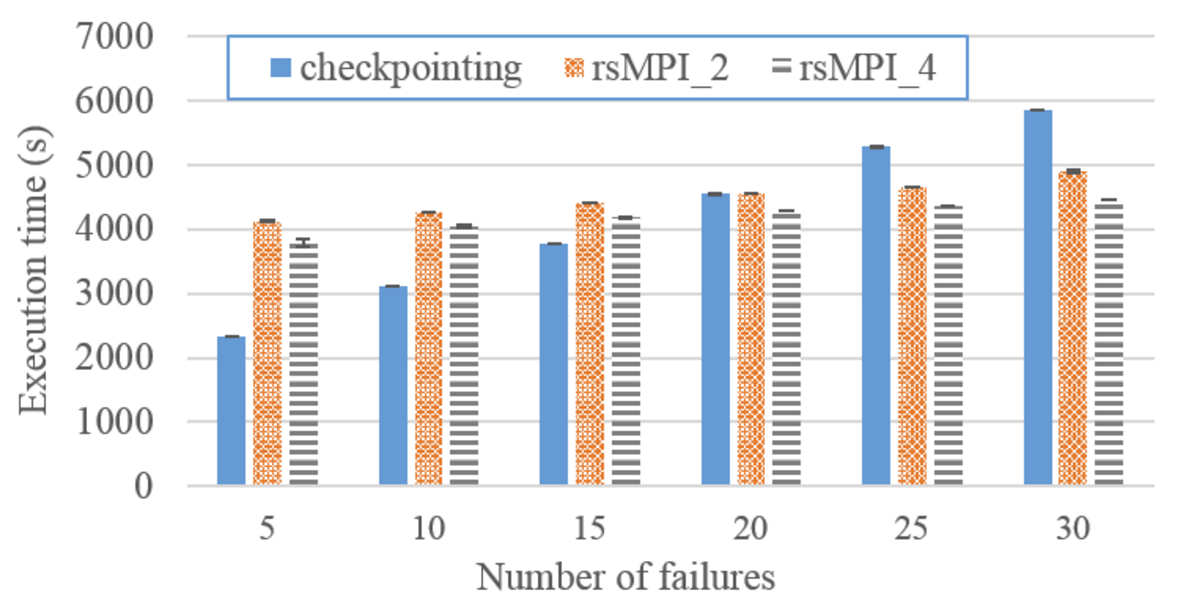
\includegraphics[width=0.9\columnwidth]{Figures/failures_ntime_hpcc}
		}
  \end{center}
  %\vskip -0.2in
  \caption{Comparison between checkpointing and rsMPI with various number of failures injected to HPCCG. 256 application-visible processes, 10\% checkpointing interval.}
  \label{fig:multiple_failure}
  \vskip -0.2in
\end{figure}


%Careful analysis of Figure~\ref{fig:failures_time} reveals that, as the number of failures increases, checkpointing and rsMPI exhibit different performance behaviors with respect to wall-clock execution time. As expected, the execution time for checkpointing increases proportionally with the number of failures. For rsMPI, however, the increase is sub-linear. This is due to fact that as more failures occur, the interval between failures is reduced, and as a result, the recovery time per failure is also reduced. Although not shown in Figure~\ref{fig:failures_time}, rebooting time will eventually dominate the recovery time when more failures occur, resulting in a linear increase in execution time for rsMPI. This increase, however, occurs at a significantly slower rate than checkpointing.

Incorporating hardware overhead, Figure~\ref{fig:failures_ntime} compares the weighted execution time between checkpointing and rsMPI.  As expected, checkpointing is better when the number of  failures is small (e.g., 5 failures).  When the number of failures increases,  however, checkpointing loses its advantage quickly. At 30 failures, for example, rsMPI\_2 and rsMPI\_4 are 19.3\% and 31.3\% more efficient than  checkpointing, respectively.
Note that, when comparing rsMPI\_2 and rsMPI\_4, the former shows higher performance with respect to wall-clock execution time, while the latter is better with respect to weighted execution time. 
%execution time is xx faster than checkpointing. It is projected to beat checkpointing in efficiency when 40 failures.
